\chapter{Contexte général}

\section{Introduction}
Aujourd'hui, de plus en plus d'administrations publiques utilisent des algorithmes et des systèmes d'IA dans leurs processus : attribution de prestations, détection de fraude, tri de dossiers, etc. Ces outils apportent de l'efficacité, mais ils créent aussi des risques concrets : un algorithme peut être biaisé, opaque, ou produire des décisions difficiles à contester.

Le problème, c'est qu'il n'existe pas d'outil simple qui permette à une organisation de répondre à ces questions :
\begin{itemize}
    \item À quel point sommes-nous exposés aux risques algorithmiques ?
    \item Avons-nous les moyens (humains, techniques, juridiques) d'y faire face ?
    \item Si on met en place un mécanisme de protection, quel sera son impact réel ?
\end{itemize}

C'est dans ce contexte que notre encadrant, Pr. B. BOUNABAT, a défini le cadre de la \textbf{PAGe Platform} : une plateforme qui permet de mesurer ces risques, d'évaluer les capacités de mitigation et de simuler l'impact des actions correctives. Le terme PAGe désigne la \textbf{Gouvernance Algorithmique Publique} (\textit{Public Algorithmic Governance}).

\section{Présentation de la plateforme PAGe}
La PAGe Platform est organisée autour de trois modules complémentaires :

\begin{itemize}
    \item \textbf{O-PAGe} (Observatoire) : ce module mesure la \textit{gravité} des risques. Chaque risque est décrit par des indicateurs quantifiables, dont les valeurs sont normalisées puis agrégées en un \textit{Risk Score}. Selon le score obtenu, le risque est classé en quatre niveaux : Low, Moderate, High ou Critical.

    \item \textbf{M-PAGe} (Mitigation) : ce module évalue la \textit{capacité de l'organisation} à atténuer ses risques. Il s'appuie sur six piliers de gouvernance (Governance, Organizational, Legal, Technical, Human, Financial), chacun décomposé en dimensions, facteurs et items de questionnaire. Le calcul agrège les réponses pour produire des scores de maturité (RL, RMMC, RMC) et un score global (GPM).

    \item \textbf{I-PAGe} (Impact) : ce module permet de \textit{simuler} l'effet du déploiement des mécanismes de mitigation sur les indicateurs de risque. Il utilise une matrice d'impact et recalcule le Risk Score après mitigation, permettant une comparaison \textit{before/after}.
\end{itemize}

\begin{figure}[H]
\centering
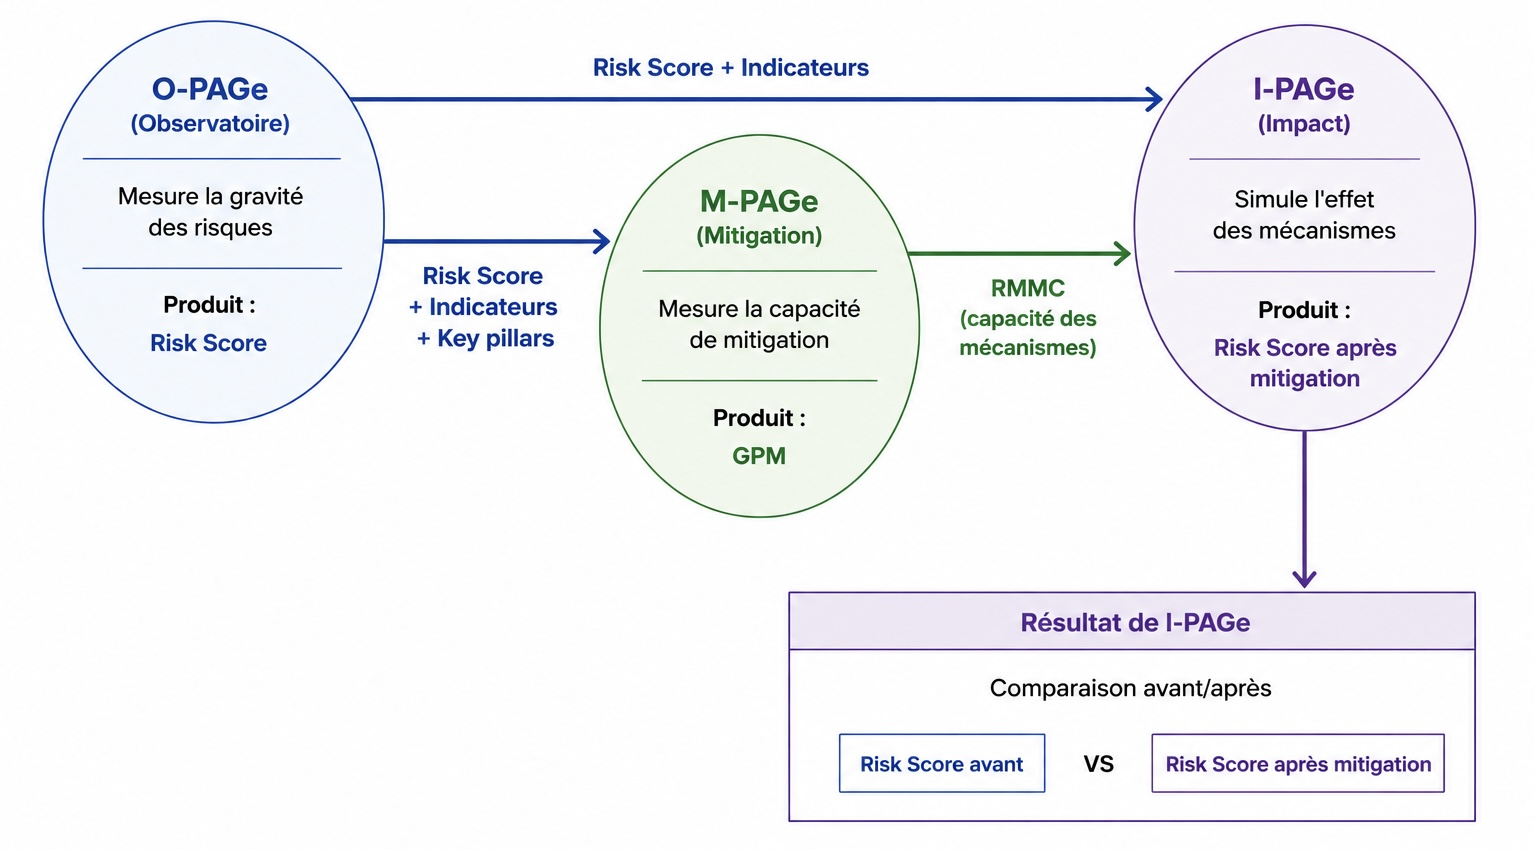
\includegraphics[width=\textwidth]{figures/schema_modulaire.png}
\caption{Architecture modulaire de la PAGe Platform}
\end{figure}
\section{Problématique}
Sans un outil adapté, l'évaluation des risques algorithmiques reste subjective et non comparable d'une organisation à une autre. Chaque institution fait sa propre appréciation, souvent qualitative, sans lien avec une mesure de sa capacité réelle à atténuer ces risques.

Notre problématique est donc la suivante : \textit{comment concevoir et développer une plateforme qui permette d'évaluer les risques algorithmiques de manière mesurable et comparable, d'apprécier la capacité de mitigation d'une organisation, et de simuler l'impact des mécanismes de réduction du risque ?}
\section{Objectifs du projet}
L'objectif global est de concevoir et réaliser la PAGe Platform comme un outil opérationnel couvrant les trois dimensions : gravité, capacité et impact.

Le projet est mené par deux binômes. Notre binôme a pour objectifs spécifiques :
\begin{itemize}
    \item développer le module \textbf{O-PAGe} en entier : gestion des risques, des indicateurs, normalisation, calcul du Risk Score, affichage des résultats ;
    \item développer la partie \textbf{front-end du module I-PAGe} : interface de simulation et visualisation before/after ;
    \item concevoir la base de données O-PAGe ;
    \item contribuer au travail commun : conception, architecture, UML.
\end{itemize}
\section{Répartition du travail}
Le travail est réparti comme suit :

\begin{table}[h]
\centering
\renewcommand{\arraystretch}{1.35}
\begin{tabular}{@{}p{0.22\textwidth}p{0.70\textwidth}@{}}
\hline
\textbf{Responsable} & \textbf{Périmètre} \\
\hline
\textbf{Binôme 1}\newline (O. AIT ELKABIR,\newline A. AL OUMAMI) &
    Module O-PAGe complet.\newline
    Front-end du module I-PAGe.\newline
    Base de données O-PAGe. \\
\hline
\textbf{Binôme 2}\newline (H. ABBAR, A. LABHAL) &
    Module M-PAGe complet.\newline
    Back-end du module I-PAGe.\newline
    Base de données M-PAGe. \\
\hline
\textbf{Travail commun} &
    Architecture globale, diagrammes UML, modèle de données.\newline correction de bugs, Démonstration. \\
\hline
\end{tabular}
\caption{Répartition du travail entre les deux binômes}
\end{table}
\section{Méthodologie de travail}
Nous avons suivi une démarche itérative, découpée en trois lots :

\begin{itemize}
    \item \textbf{Lot 1 --- Analyse et conception :} comprendre le besoin, définir les cas d'usage, faire la modélisation UML, concevoir les interfaces et la base de données, comprendre les règles de calcul.
    \item \textbf{Lot 2 --- Développement :} coder les 3 Modules, implémenter les calculs, intégrer la base de données.
    \item \textbf{Lot 3 --- Tests et soutenance :} préparer la démo et le rapport.
\end{itemize}

À chaque lot, on validait avec l'encadrant avant de passer à la suite. À l'intérieur de chaque lot.
\section{Planning}
Le projet s'est déroulé sur environ trois mois (12 semaines) :

\begin{table}[h]
\centering
\renewcommand{\arraystretch}{1.3}
\begin{tabular}{@{}p{0.16\textwidth}p{0.62\textwidth}p{0.14\textwidth}@{}}
\hline
\textbf{Période} & \textbf{Activités} & \textbf{Lot} \\
\hline
Semaine 1 & Cadrage fonctionnel, identification des acteurs, répartition des tâches, diagramme de cas d'usage. & Lot 1 \\
\hline
Semaines 2--3 & Diagramme de classes, base de données, maquettes d'interfaces, spécification des API. & Lot 1 \\
\hline
Semaines 4--5 & Configuration BD, authentification, développement O-PAGe (indicateurs, normalisation, Risk Score). & Lot 2 \\
\hline
Semaines 6--7 & Développement M-PAGe (KP, dimensions, facteurs, items, calculs RL/RMMC/RMC/GPM). & Lot 2 \\
\hline
Semaines 8--9 & Développement I-PAGe (matrice d'impact, efficacité RMM, recalcul Risk Score). & Lot 2 \\
\hline
Semaines 9--10 & Intégration des 3 modules, correction de bugs. & Lot 3 \\
\hline
Semaine 11 & Tableaux de bord, exports PDF/Excel, documentation. & Lot 3 \\
\hline
Semaine 12 & Préparation soutenance et démo, finalisation rapport. & Lot 3 \\
\hline
\end{tabular}
\caption{Planning du projet}
\end{table}
\vspace{10cm}
\section{Conclusion}
Ce chapitre a posé le contexte du projet, formulé la problématique et précisé nos objectifs et notre périmètre de travail. Le chapitre suivant présente le cadre conceptuel de la plateforme : les définitions des concepts clés et les formules de calcul qui fondent les trois modules.